An assurance is an AIA property or behavior that can either increase or decrease user trust. The term `assurances' is perhaps earliest used in the context of human-AIA relationships by \citet{Sheridan1984-kx}. \citet{McKnight2001-fa} allude to this kind of feedback in e-commerce relationships as `Web Vendor Interventions'. \citet{Corritore2003-gx} refer to assurances as `trust cues' that can influence how online users trust e-commerce vendors. \citet{Lee2004-pv} discuss `display characteristics', which are methods by which an autonomous systems can communicate information to an operator. More recently, \citet{Lillard2015-yg} provided a formal definition of assurances for autonomous systems that is similar to the one used here. 

\begin{figure}[t]%[htpb]
    \centering
    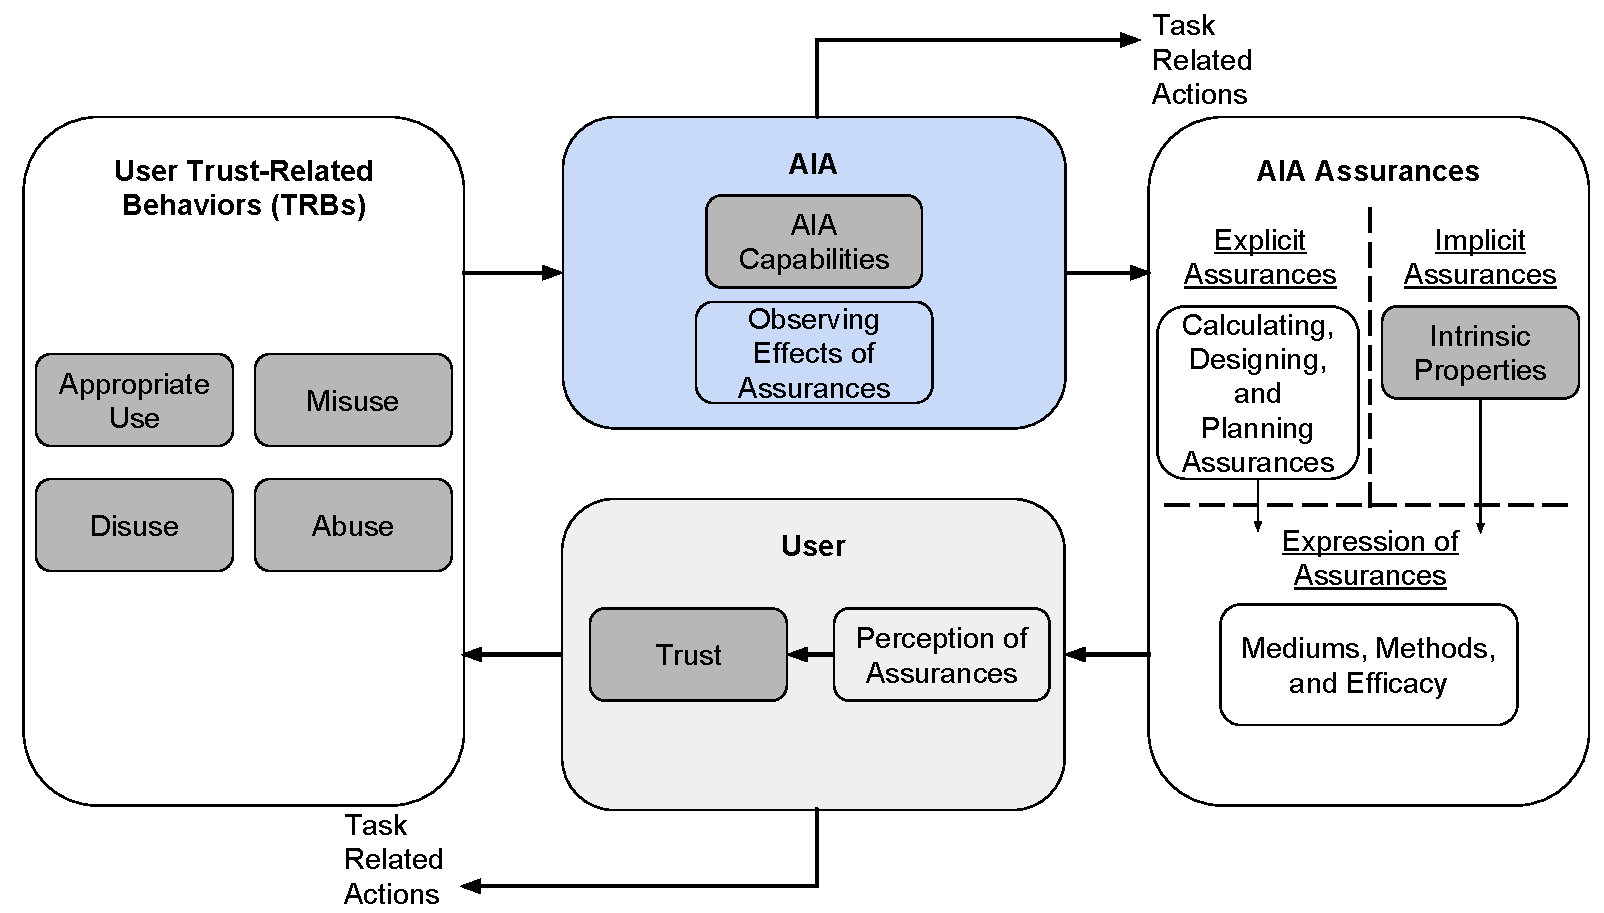
\includegraphics[width=0.6\linewidth]{Figures/RefinedTrust_one_way.pdf}
    \caption{Figure depicting the details of the human-AIA trust cycle.}
    \label{fig:refined_trust}
\end{figure}

Assurances can be classified in several different ways. One way to classify an assurance is by its \emph{Information Source:}. Assurances must be informed by some kind of information, whether that means real-time observation of TRBs in order to have feedback, or well accepted concepts of cognitive science as guiding principles of design.
Another approach is to identify the \emph{Source/Target} pair: In a human-AIA trust relationship, assurances link the AIA to the user. The user has multi-dimensional trust in the AIA (see Fig.~\ref{fig:Assurance_classes}), and each AIA capability has multiple dimensions of `trustworthiness'. In designing an assurance it is useful to explicitly identify the source capability, and the target trust dimension (i.e. a certain assurance may have been designed as a `planning-competence').
An assurances can be considered \emph{Component} or \emph{Composite:} A component assurance stems from one AIA capability to one trust dimension. A composite assurance originates from multiple AIA capabilities to one trust dimension.
Another consideration is whether the assurance is \emph{Tutoring} or \emph{Telling:} An assurance that is dynamic to the different characteristics, and experience of users is a `tutoring' assurance. It is designed to help a user learn, over time, to trust appropriately. Conversely, all other assurances are `telling' in that they are static in regards to separate users.
\emph{Mode of Expression:} Assurances can also be classified by their mode of expression. This includes the method and medium by which the assurance is expressed.
There are many open questions regarding each of these categories; they are discussed further in Sec.~\ref{sec:future_work}, regarding future work.

\emph{Level of Integration:} Herein the `level of integration' of assurances are surveyed. This is useful because it addresses a natural consideration in the design process of AIAs; it also encapsulates well the key approaches that are in use. In this context `integration' refers to the level of effect the assurance has on the core functions of the AIA. As an example: an assurance that, if missing, greatly effects the AIA functionality is considered integral to the AIA. Conversely, a missing assurance that has no effect on the AIA functionality is not integral; we also call this `supplemental'. Between these two extremes there is a natural continuum of integration on which we can classify the different algorithmic approaches to designing assurances; we do so in Sec.~\ref{sec:synthesis}.
